\documentclass[letterpaper,10pt]{article}
%paquetes
\usepackage[spanish, es-tabla]{babel}%formato de las tablas
\usepackage[utf8]{inputenc}
\usepackage{enumerate}
\usepackage{graphicx}
\usepackage{float}
\usepackage[T3,T1]{fontenc}
\usepackage{amsmath,wasysym,amssymb,amsfonts,textcomp,latexsym}
\usepackage{hyperref}
\usepackage{appendix}
\usepackage{enumitem}
\usepackage[ruled,vlined,lined,linesnumbered,algosection,spanish]{algorithm2e}
\usepackage{multimedia}
%\usepackage[intlimits]{amsmath}
\usepackage{flexisym}
\usepackage{xparse}
\usepackage{mathtools}
\usepackage{bm}
\usepackage{draftwatermark}

\SetWatermarkText{\textsc{Borrador}}
\SetWatermarkScale{5}
\SetWatermarkAngle{55}
%%%
% \usepackage{ragged2e}
% \usepackage{pstricks,enumerate}

%\setpapersize{A4}
% Numeración
%\usepackage{vmargin}
%\setmargins{1.5cm}       % margen izquierdo
%{1.5cm}                        % margen superior
%{16.5cm}                      % anchura del texto
%{23.42cm}                    % altura del texto
%{10pt}                           % altura de los encabezados
%{1cm}                           % espacio entre el texto y los encabezados
%{0pt}                             % altura del pie de página
%{2cm}                           % espacio entre el texto y el pie de página
\setcounter{secnumdepth}{30}
\title{Propuesta Alberto Rodríguez Sánchez}

\begin{document}
\renewcommand{\refname}{Bibliografía}%%pone en lugar de referencias bibliografía esta dentro porque se ocupap babel en otro caso iria afuera.
% Pagina sin estilo para portada quitar encabezado, pie y número de página
\thispagestyle{empty}

\begin{center}
    {\Huge Universidad Autónoma Metropolitana }\\
    {\huge Unidad Azcapotzalco}\\
    \vspace{0.5cm}
    {\Large División de Ciencias Básicas e Ingeniería}\\
    \vspace{1.0cm}
    {\large Posgrado en Optimización}\\
    \vspace{2.0cm}    
    {\Large TODO}\\
    \vspace{1.0cm}
    {\large Propuesta de Proyecto de Investigación}\\
    \vspace{2.0cm}
    {\large\textbf{Alumno:}}\\
    Alberto Rodríguez Sánchez\\
    %\bigskip 2153800510\\
    \vspace{1.5cm}
    \bigskip
    {\large\textbf{Asesores:}}\\
    Dr. Antonin Ponsich Sebastien\\
    \vspace{1.5cm}
     2017\\
    \vspace{1.0cm}
    Ciudad de México\\
\end{center}
\newpage
\tableofcontents
\newpage
\section{Introducción}

El problema de optimización multiobjetivo \textbf{(MOP)} ha sido de gran interés en la comunidad científica e industrial; ya que, es común encontrar problemas que requieren considerar múltiples objetivos incluyendo tiempo, costos, cantidad, calidad, etc, donde estos objetivos se encuentran en conflicto y se puede encontrar inmerso en diferentes problemas como: ruteo de vehículos, localización, cadenas de suministro, calendarización, entre otros. Desde el punto vista Metaheurístico se han generado tres grandes ramas para resolver el \emph{MOP}:

\begin{itemize}
 \item Descomposición
 \item Dominancia
 \item Métricas
\end{itemize}

El enfoque de descomposición explícitamente descompone un problema multiobjetivo en $N$ problemas de optimización escalares y suele introducir técnicas poblacionales para la resolución simultánea de ellos, es importante seleccionar los problemas escalares conforme a algún criterio que permita mejorar la diversidad, dejando la convergencia al sub método de resolución.Un marco de trabajo moderno con este enfoque es \emph{MOEA/D}.
\newline

En el enfoque de dominancia se utilizan las relaciones de dominancia de Pareto para inducir un orden parcial en el espacio de los objetivos y de esta manera decidir cuándo una solución en dicho espacio es comparable con otra y de serlo cual es mejor, dicho orden parcial está limitado en espacios de altas dimensiones puesto que gran cantidad de soluciones seran no comparables merma la efectividad de los procedimientos de selección. \emph{NSGA-III} un marco de trabajo moderno con este enfoque incorpora técnicas de nichos para sortear este problema.
\newline

El enfoque de métricas convierte el problema multiobjetivo en un problema mono objetivo que maximiza el valor de métricas que permitan definir si el conjunto de soluciones es de buena calidad y  tiene buena dispersión, una métrica popular es el hipervolumen ya que permite saber al mismo tiempo si se tiene cierta convergencia y dispersión. Sin embargo, calcular estas métricas se vuelve costoso conforme aumentan las dimensiones del problema multiobjetivo original, por ejemplo, la mejor forma conocida de calcular el hipervolumen tiene una complejidad de $O(n^2m^3)$ donde $n$ es el número de puntos en el frente y $m$ las dimensiones de los mismos.
\newline

Es importante hacer notar ... \emph{Ideas sobre los enfoques de descomposición y dominancia y los la geometría del  simplejo y los nichos??}
\newline

{\huge TODO}

\subsection{Estado del arte del \emph{MOP}}

El Problema de Optimización Multiobjetivo (MOP) (llamado también
multicriterio o vectorial) puede definirse como el problema de
encontrar (Osyczka, 1985)\cite{Osyczka1985193}:
\begin{quote}
Un vector de variables de decisión que satisfacen un cierto
conjunto de restricciones y optimice un conjunto de funciones
objetivo. Estas funciones forman una descripción matemática
de los criterios de desempeño que suelen estar en conflicto
unos con otros y que se suelen medir en unidades diferentes.
El término ``optimizar'' en este caso toma pues un significado
diferente al del caso de problemas mono-objetivo.
\end{quote}

\subsection{Formulación Matemática}
El problema de Optimización Multiobjetivo (MOP) se define en su forma general de la siguiente manera:
 
$$\min \overrightarrow{F(\bm{x})} = \left[ \overrightarrow{f_1(\bm{x})}, \overrightarrow{f_2(\bm{x})} , \dots, \overrightarrow{f_n(\bm{x})} \right] $$
S.A:
 
$$g_i(\bm{x}) \leq 0, i=1,2,\dots,m$$
$$h_i(\bm{x}) = 0, i=1,2,\dots,p$$
 
Buscamos el vector $\bm{x}=[x_1,x_2,\dots,x_k]^T$ que optimice la función $\overrightarrow{F}$

\newpage
 
\subsection{Métodos empleados para resolver el MOP mejorando la diversidad de las soluciones}

Por ser el \emph{MOP} un problema ampliamente estudiado se han propuesto varios algoritmos para generar vectores de pesos iniciales en el caso del enfoque de descomposición como:
\newline

{\huge TODO}

% Siwei Jiang y Jie Zhang (2011) proponen un algoritmo de  \cite{mie99}, Karabakal N. et al., (1993), proponen un método de ajuste del multiplicador de pendiente más pronunciado \cite{4358754}, Savelsbergh M. (1997) presenta ún algoritmo de ramificación y precio \cite{4358754}, I.R. de Farias et al. (2000) proponen una aproximación poliedral y muestran que cortan todos los vértices infactibles de la relajación del problema lineal y demuestran la superioridad del método de ramificación y corte sobre el de ramificación y acotamiento \cite{4358754}, entre otros.
% \newline
%
%
%
% También, heurísticas han sido propuestas para resolver el \emph{PAG}:
% \newline
%
% Martello, S. y P. Toth (1981) proponen una búsqueda glotona con búsqueda local \cite{4358754}, Mazzola (1989) describe una asignación generalizada con interacción de capacidad no lineal y un algoritmo heurístico en dos fases, donde la primera fase busca identificar una solución factible para la versión no lineal del PAG (NLPAG) y la segunda intenta mejorar la calidad de la solución a NLPAG  \cite{4358754}, Trick M.A. (1989) examina la estructura básica de la relajación lineal y muestra que hay más información disponible, esto conduce a una prueba alternativa del teorema de Benders y Van Neunen y emplean una heurística para el problema de asignación generalizada, para la generación de restricciones que generen límites inferiores para encontrar mejores soluciones \cite{4358754}, otras propuestas están en \cite{4358754}, \cite{4358754}.     
% \newline
%
% Algunos métodos híbridos han sido propuestos para resolver el \emph{PAG} e.g:
% \newline
% Klastorin (1979) desarrolló un algoritmo heurístico de dos etapas utilizando un enfoque de subgradiente modificado y la estrategia de ramificación y acotamiento para resolver el problema de asignación generalizada \cite{4358754}, Fisher et al. (1986) describen un algoritmo de ramificación y acotamiento en el cual las cotas son obtenidas por una relajación lagrangiana con los conjuntos multiplicadores por un método de ajuste heurístico \cite{4358754}, Guignard M. et al. (1989) proponen un algoritmo basado en una improvisacion dual donde el rendimiento mejorado proviene de un productor de ascenso dual lagrangiano mejorado que resuelve un dual lagrangiano en cada nodo de enumeración añadiendo una restricción al modelo relajado lagrangiano y un elaborado esquema de ramificación y acotamiento \cite{4358754}, entre otros.
%      
\section{Justificación}

% Debido a que el \emph{PAG} pertenece a la clase NP-Duro \cite{4358754}; ha sido  resuelto por diferentes métodos heurísticos con el fin de obtener una solución en un tiempo razonable.
%
Las metaheurísticas son técnicas de solución versátiles, flexibles y eficientes, estos algoritmos pueden resolver problemas complejos de optimización multiobjetivo \cite{coello1999comprehensive} .
\newline
%
%  En la actualidad muchas heurísticas han surgido inspiradas por diferentes características de algún tipo  de comportamientos social o agentes diversos en la naturaleza, un subconjunto de estas ha sido desarrollado por imitación de las llamadas inteligencia de enjambre (SI) tales como aves y peces entre otros. La optimización  de enjambre de partículas se basó en el comportamiento de aves y peces \cite{4358754}, mientras que el algoritmo de luciérnagas se basó en el patrón intermitente de las luciérnagas tropicales \cite{4358754}, \cite{4358754}.
% \newline
%      
% Los algoritmos de luciérnagas (FA), gravitación universal (GSA) y el método de composición musical (MMC), los cuales fueron diseñados para ser aplicados a problemas de optimización continua,  han sido adaptados para problemas de optimización discreta \cite{4358754}, \cite{4358754}, \cite{4358754}.
% Para el \emph{PAG} aún no han sido implementados estos tres métodos heurísticos, es por esa razón que se utilizarán en este trabajo con el fin de reportar su comportamiento, así mismo se compararán con algunas de las técnicas de las existentes en la literatura, en cuestión de calidad de la solución y tiempo de respuesta; para este trabajo se utilizarán las instancias de P. C. Chu y J. E. Beasley planteados en \cite{4358754}, los archivos se encuentran disponibles en \textbf{OR-Library} \cite{4358754}.

\section{Objetivo General}

Adaptar los métodos heurísticos MOEA/D y NSGA-III para resolver algunas instancias de prueba, las cuales se encuentran disponibles en \cite{zhang2008multiobjective} y comparar los resultados obtenidos con algunos reportados en la literatura.

\section{Objetivos Particulares}

\begin{itemize}
\item Desarrollar al menos una estrategia para generar vectores iniciales de buena calidad para \emph{MOEA/D} en el conjunto de instancias propuestas en \cite{zhang2008multiobjective}.

\item Desarrollar al menos una estrategia de actualización de vectores de pesos para el método \emph{MOEA/D}.

\item Desarrollar al menos una estrategia para generar puntos de referencia iniciales de buena calidad para \emph{NSGA-III} en el conjunto de instancias propuestas en \cite{zhang2008multiobjective}.

\item Desarrollar al menos una estrategia de actualización de puntos de referencia para el método \emph{NSGA-III}.

\item Integrar la estrategia de repulsion de subpoblaciones\cite{ahrari2016multimodal} a los métodos \emph{MOEA/D} y \emph{NSGA-III}.

\item Adaptar, implementar y describir el comportamiento del método \emph{MOEA/D} para las instancias seleccionadas.
 
\item Adaptar, implementar y describir el comportamiento del método \emph{NSGA-III} para las instancias seleccionadas.

\item Comparar los resultados obtenidos de las dos heurísticas con algunos resultados obtenidos en la literatura.

\item Identificar las ventajas y desventajas de los algoritmos implementados con respecto a las métricas de diversidad.
\end{itemize}

\section{Marco de Trabajo MOEA/D}
El \emph{MOEA/D} fue desarrollado por Qingfu Zhang y Hui Li de la Universidad de Essex en 2007. \cite{4358754}
 
Es un algoritmo de optimización inspirado en las técnicas de descomposición y los algoritmos genéticos, que se basa en el descomponer un problema multiobjetivo en $N$ problemas de optimización escalares y resolverlos simultáneamente, de esta manera se caracteriza por tener las siguientes características
 \begin{itemize}
 \item Tecnicas de analisis geometrico sobre el simplejo del problema \cite{mie99,Das:1998:NIN:588907.589322, Messac2003}
 \item Mejora de soluciones hasta óptimos locales/globales garantizados por el teorema de Holland\cite{Holland:1992:ANA:531075}
 \end{itemize}
 
Existen cuestiones importantes del \emph{MOEA/D} asociado con la geometria del problema de programación no lineal \cite{4358754}:

% \begin{itemize}
% \item La variación de la intensidad de la luz o el brillo I(r) varía de acuerdo a la ley del inverso cuadrado.
% \begin{equation} I(r)= \frac{I_{s}}{r^{2}} \end{equation}
% \item Donde $I_{s}$ es la intensidad de la fuente, para una media dada con un ajuste del coeficiente de absorción de luz  \emph{$\gamma$}, la intensidad de la luz \emph{I} varía con la distancia \emph{r}=. Esto es      
% \begin{equation} I= I_{0}{e^{\gamma r}} \end{equation}
% \item Donde $I_{0}$ es la intensidad de luz original, en el caso singular donde $r=0$  en la expresión  $I(r)= \frac{I_{s}}{r^{2}}$, el efecto combinado de la ley del cuadrado inverso y la absorción puede aproximarse de la siguiente forma Gaussiana.
% \begin{equation} I= I_{0}{e^{\gamma r^{2}}}  \end{equation}
% \item La formulación de atractivo \begin{math}\beta\end{math}
%
% \begin{equation} \beta= \beta_{0}{e^{\gamma r^{2}}}\end{equation}
%
%
% \item La distancia entre dos luciérnagas cualesquiera \emph{i} y \emph{j} y respectivamente  $x_{i}$ y $x_{j}$, es la distancia cartesiana.
%
% \begin{equation} r_{i,j}= ||x_{i} - x_{j}||= \sqrt{ \sum_{k=1}^{d}(x_{i,k} - x_{j,k})}\end{equation}
% \end{itemize}
% En \cite{yang2010nature} idealizan las características de los destellos de las luciérnagas para desarrollar el \emph{FA}.
%
% El movimiento de una luciérnaga \emph i con localización \begin{math}x_{i}\end{math} atraída por otra luciérnaga j más brillante y localización \begin{math}x_{j}\end{math} está determinada por:
% \begin{center}
% \begin{equation} x_{i}(t+1)=x_{i}(t)+ \beta_{0}{e^{\gamma {r_{i,j}^2}}}(x_{j} - x_{i})+\alpha\varepsilon_{i} \end{equation}
% \end{center}


\subsection{Pseudocódigo MOEA/D}

 \centering
   \scalebox{.85}{
    \begin{algorithm}[H]
   \caption{Algoritmo MOEA/D}
   %\SetLine
    \KwData{$IterMax$: condición de paro, $N$:subproblemas a considerar, $T$: Tamaño de vecindario, $P_{crossover}$, $P_{mutation}$}
    \KwResult{$PE$:Frente Aproximado}
Poblacion $\leftarrow$ PoblacionInicial($Poblacion_{size}$, $NumObjetivos$)\;
 
$W = {\bm{w}_1,\dots,\bm{w}_N}$ $\leftarrow$ VectoresDePesosUniformementeDistribuidos(N)\;
${B_0,\dots,B_N} \leftarrow$ VecinosCercanos($T$, $W$)\;
 
\While {$\neg$Paro($IterMax$)}{
 
\For {$i:=1$ a $N$}{
Selección $\leftarrow$ SeleccionPadres($B_i$)\;
$C_i$ $\leftarrow$ CruzayMutacion(Selección, $P_{crossover}$, $P_{mutation}$)\;
\If {$C_i \preceq x \in B_i$}{
$x$ $\leftarrow$ $C_i$\;}
}
$PE$ $\leftarrow$ ActualizarPE($Poblacion$)
}
 
\Return($PE$)
\end{algorithm}}

\section{Marco de Trabajo NSGA-III}

El marco de trabajo \emph{NSGA-III} fue propuesto por K. Deb and H. Jain en 2014.\cite{6600851}, es una mejora a NSGA-II para trabajar con problemas de más de  $3$ funciones objetivos. propone sustituir “Crowding distance” por métodos de nichos de tal manera que ayuden a mejorar la diversidad de la población.

{\huge TODO}

% La ley de Gravitación Universal fue publicada en 1687 por Isaac Newton. El \emph{GSA} fue introducido por Esmat Rashedi et al. (2009) \cite{4358754} donde se muestra un algoritmo de búsqueda poblacional basado en las reglas de la gravitación universal donde se da una breve descripción de la fuerza gravitacional para proporcionar un medio apropiado y seguido por la explicación de \emph{ GSA}.  
%
% \subsection{Ley de la gravitación}
% La gravitación es la tendencia de las masas a acelerar  una hacia otra, esta es una de las cuatro fundamentales interacciones en la naturaleza (las otras son: la fuerza electromagnética, la fuerza nuclear débil y la fuerza nuclear fuerte). Por lo que, cada partícula en el universo atrae a cualquier otra partícula con una ``fuerza gravitacional'' \cite{rashedi2009gsa}.
% \newline
%
% La forma de la fuerza gravitacional de Newton es llamada ``acción distancia'', significa cambios de gravedad entre partículas separadas sin cualquier intermediario y sin demora alguna.
% \newline
%
%  La fuerza gravitacional entre dos partículas es directamente proporcional al producto de sus masas $M_{1}$ y $M_{2}$ e inversamente proporcional al cuadrado de las distancias R entre ellas.
% \newline
% \begin{equation}F= \frac{GM_1M_2}{R^2}\end{equation}
% \newline
%
% Donde \emph{F} es la magnitud de la fuerza gravitacional, \emph{G} es la constante gravitacional, \emph{$M_{1}$} y  \emph{$M_{2}$} son las masas de la primera y segunda partícula respectivamente y \emph{R} es la distancia entre las dos partículas.
% \newline
%
%  La segunda ley de Newton dice que cuando una fuerza, ``F'', es aplicada a una partícula, su aceleración ``a'', depende sólo de la fuerza y su masa ``M". \newline
%  \begin{equation}a= \frac{F}{M}\end{equation}
%  \newline
%
%  Hay una fuerza de atracción entre todas las partículas del universo, donde el efecto de la partícula  más grande y la partícula más pequeña es mayor, por lo que, un incremento en la distancia entre dos partículas significa decrecimiento en la fuerza de gravedad entre ellas.\newline
%  
%  Debido al efecto de disminuir la gravedad, el valor actual de la constante gravitacional depende del estado actual del universo, la siguiente fórmula describe     el decrecimiento de la constante gravitacional, ``G'', con el estado:
%
% \begin{equation} G(t)=G(t_{0})x(\frac{t_{0}}{t})^\beta, \text{ } \text{ }\beta <1\end{equation}
%
% Donde \emph{$G(t)$} es el valor de la constante gravitacional en el tiempo t, \emph{$G(t_{0})$} es el valor de la constante gravitacional en el intervalo de tiempo \emph{$t_{0}$}.
% \newline
%
% En el \emph{GSA} cada masa(Agente) tiene cuatro especificaciones:
% \begin{itemize}
% \item[] a) Posición, b) Masa de inercia, c) Masa gravitacional activa, d) Masa gravitacional pasiva.
% \end{itemize}
%
% La posición de la masa corresponde a una solución del problema y las masas de inercia y gravitacional son determinadas utilizando la función objetivo o función aptitud, en otras palabras cada masa representa una solución y el algoritmo navega ajustando correctamente las masas gravitacionales y la inercia, con el transcurso de tiempo, esperando que las masas sean atraídas por las masas más pesadas, éstas representan una mejor solución en el espacio de búsqueda.
%
\subsection{Pseudocódigo NSGA-III}
% \centering
%     \scalebox{.65}{
%      \begin{algorithm}[H]
%     \caption{Algoritmo NSGA-III}
%     
% \KwData{$K$:puntos de referencia estructurados $\bm{Z}^{(K)}$, $NumObjetivos$, $P_{crossover}$, $P_{mutation}$}
% \KwResult{$Hijos$}
%  Poblacion $\leftarrow$ InitializePoblacion($Poblacion_{size}$, ProblemSize)\;
%  EvaluateAgainstObjectiveFunctions(Poblacion)\;
%  FastNondominatedSort(Poblacion)\;
%  Seleccion $\leftarrow$ SelectPadresByRank(Poblacion, $Poblacion_{size}$)\;
%  Hijos $\leftarrow$ CrossoverAndMutation(Seleccion, $P_{crossover}$, $P_{mutation}$)\;
%  \While{$\neg$Paro()}{
%  EvaluateAgainstObjectiveFunctions(Hijos)\;
%  Union $\leftarrow$ Merge(Poblacion, Hijos)\;
%  Frentes $\leftarrow$ FastNondominatedSort(Union)\;
%  Padres $\leftarrow \emptyset$\;
%  $Frente_L$ $\leftarrow \emptyset$\;
%  \For {$Frente_i$ $\in$ Frentes}{
%   Niching($Frente_i$)\;
%  \eIf{$Size(Padres)+Size(Frente_i) > Poblacion_{size}$}{
%  $Frente_L$ $\leftarrow$ $i$\;
%  Break()\;
%  }
%  }
%   Padres $\leftarrow$ Merge(Padres, $Frente_i$)\;
%  \If {$Size(Padres) < Poblacion_{size}$}{
%  $Frente_L$ $\leftarrow$ SortByRankAndDistance($Frente_L$)\;
%  \For {$P_1$ To $P_{Poblacion_{size} - Size_{Frente_L}}$}{
%  Padres $\leftarrow$ $Pi$
%  }
%  }
%  Seleccion $\leftarrow$ SelectPadresByRankAndDistance(Padres, $Poblacion_{size}$)\;
%  Poblacion  $\leftarrow$ Hijos\;
%  Hijos $\leftarrow$ CrossoverAndMutation(Seleccion, $P_{crossover}$, $P_{mutation}$)\;
% }
%  \Return (Hijos)
% \end{algorithm}}
\begin{figure}[h]
 \centering
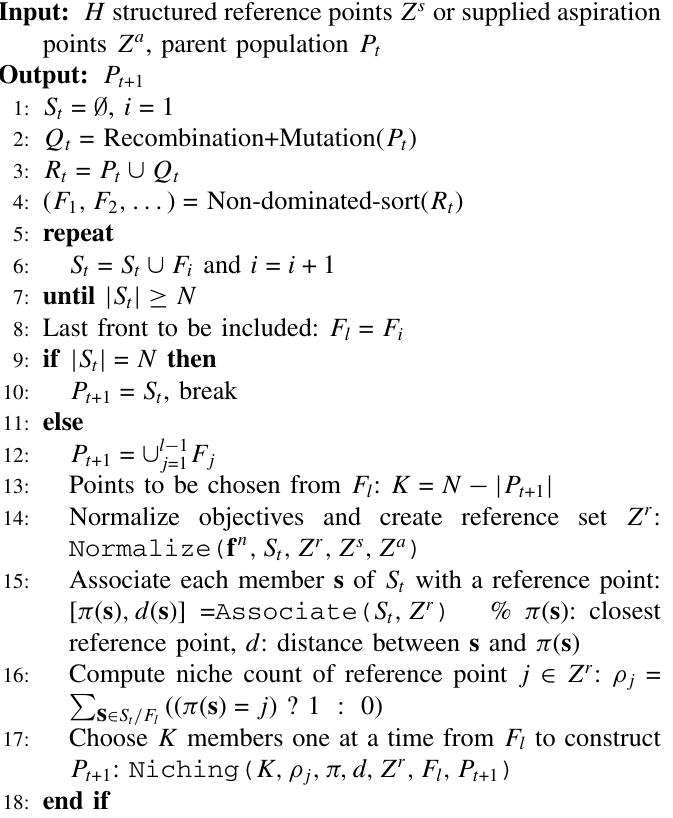
\includegraphics[scale=0.35]{nsgaiiiP.png}
\end{figure}

\section{Metodología}

Para la implementación de las dos heurísticas basadas en los enfoques de descomposición y dominancia, se ha estado haciendo una revisión en el estado del arte para analizar las características de los marcos de trabajo NSGA-III y MOEA/D, tomándolas  como  base para la adaptación al problema, posteriormente se propondrán mejoras a estos algoritmos.
 
Posteriormente se realizará un análisis estadístico de cada una de las técnicas implementadas, comparando su rendimiento contra algunas de las  técnicas propuestas en la literatura.
 
 \begin{itemize}
 \item[•] \textbf{ETAPA 1.} \emph{Se analizó el estado del arte para el MOEA/D y NSGA-III identificando los aportes recientes en cuestiones de diversidad.}
\item[] Identificando y listando las técnicas reportadas en tres clases: métodos basados en descomposición, métodos basados en dominancia y métodos basados en metricas. Así mismo, se han revisado las técnicas que se busca implementar al problema analizando su estructura y características.
\emph{(Concluida)}

\item[•] \textbf{Etapa 2.} \emph{Adaptación e implementación de los marcos de trabajo MOEA/D y NSGA-III para incluir mejoras en la selección de vectores/puntos de referencia iniciales y técnicas de adaptación dinámica de los mismos.}

\item[] Con base al análisis del perfil de nuestras técnicas, se implementarán en un lenguaje de programación.
        
\item[•] \textbf{Etapa 3.} \emph{Comparaciones de las técnicas y análisis estadístico.}

\item [] Una vez que se tengan las estrategias implementadas, se realizarán comparaciones de calidad de las soluciones obtenidas por cada una y la cantidad de recursos computacionales  que utilizan. Posteriormente, se justificará su rendimiento con un análisis estadístico detallado para cada  una de estas.

\item[•] \textbf{Etapa 4.} \emph{Proceso de mejora de las técnicas.}

\item[] Las técnicas se someterán a un estudio para identificar si algunas funciones se pueden mejorar con algún cambio en la implementación, que dé como resultado disminución en el tiempo de ejecución o reducción en el costos de recursos.


\item[•] \textbf{Etapa 5.} Comparación de las técnicas definidas y reporte de resultados.

\item[] Una vez terminada la etapa de mejoras de cada una de las técnicas, se realizará un nuevo análisis estadístico para comparar el rendimiento de cada una de nuestra técnicas, describiendo los resultados obtenidos.
        
  \end{itemize}

\subsection{\textbf{Diseño de experimentos}}
Los experimentos consistirán en la medición de la calidad de las soluciones dadas por cada una de las técnicas así como de su tiempo de ejecución para un conjunto de instancias benchmark.
         
\section{Cronograma}
\begin{table}[H]
\centering

\label{my-label}
\scalebox{0.9}{\begin{tabular}{|l|c|c|c|c|}
\hline
\begin{tabular}[c]{@{}c@{}}Nombre\\   de la tarea\end{tabular} & Fecha de Inicio & Fecha final & \% Completado & Duración \\ \hline
Presentación propuesta de tesis                                & XX/XX/17        & XX/XX/17    & XXX\%         & XXd      \\ \hline
Adaptación MOEA/D con adaptación de vectores                   & XX/XX/17        & XX/XX/17    & XX\%          & XXd     \\ \hline
Adaptación NSGA-III con adaptación de puntos de referencia     & XX/XX/17        & XX/XX/17    &               & XXd      \\ \hline
Análisis y comparación de técnicas                             & XX/XX/17        & XX/XX/17    &               & XXd      \\ \hline
Redacción de tesis                                             & XX/XX/17        & XX/XX/17    &               & XXd      \\ \hline
Entrega de tesis                                               & XX/XX/17        & XX/XX/17    &               & 1d       \\ \hline
\end{tabular}
}
\caption{Cronograma}
\end{table}



\begin{table}[H]
\centering
\label{my-label}
\scalebox{0.6}{\begin{tabular}{|l|l|}
\hline
Nombre de la tarea                 & \multicolumn{1}{c|}{Metas alcanzar al terminar la tarea}                                                                                                                                                                                                                                                                                                                                                            \\ \hline
Presentación propuesta de tesis    & Aprobación de propuesta de tesis por el comité de posgrado.                                                                                                                                                                                                                                                                                                                                                         \\ \hline
Correcciones propuesta de tesis    & Registro de Aceptación de tesis.                                                                                                                                                                                                                                                                                                                                                                                    \\ \hline
Adaptación FA para el PAG          & \begin{tabular}[c]{@{}l@{}}Se busca describir el comportamiento de la técnica implementada al PAG y probada\\ con algunas instancias disponibles, esperando tener buenos resultados con respecto de\\  las técnicas existentes en la literatura,  comparando la calidad de la solución y el número\\  de llamadas a la función objetivo;  así como las ventajas y desventajas que ofrece esta técnica.\end{tabular} \\ \hline
Adaptación GSA para el PAG         & \begin{tabular}[c]{@{}l@{}}Se busca describir el comportamiento de la técnica implementada al PAG  y probada \\ con algunas instancias disponibles,  esperando tener buenos resultados con respecto de\\ las técnicas existentes en la literatura, comparando la calidad de la solución y el número\\ de llamadas a la función objetivo; así como las ventajas y desventajas que ofrece esta técnica.\end{tabular}  \\ \hline
Adaptación MMC para el PAG         & \begin{tabular}[c]{@{}l@{}}Se busca describir el comportamiento de la técnica implementada al PAG y probada \\ con algunas instancias disponibles, esperando tener buenos resultados con respecto de \\ las técnicas existentes en la literatura, comparando la calidad de la solución y el número\\ de llamadas a la función objetivo;  así como las ventajas y desventajas que ofrece esta técnica.\end{tabular}  \\ \hline
Anélisis y comparación de técnicas & \begin{tabular}[c]{@{}l@{}}Se busca describir el comportamiento de nuestras técnicas con la finalidad de poder\\ decir cuales son sus ventajas o defectos al ser utilizadas con las instancias seleccionadas\\ para el PAG.\end{tabular}                                                                                                                                                                            \\ \hline
Redacción de tesis                 & Documentación de la investigación realizada.                                                                                                                                                                                                                                                                                                                                                                        \\ \hline
Entrega de tesis                   & \begin{tabular}[c]{@{}l@{}}Obtener la\\   aprobación y fecha para el examen de grado\end{tabular}                                                                                                                                                                                                                                                                                                                   \\ \hline
\end{tabular}
}
\caption{Metas}

\end{table}

%\begin{figure}[H]
%\begin{center}
    %\scalebox{0.800}{\includegraphics{cronogramatesis.jpg}}%%%%%%%%%%%%%%%%%%Cambiar imagen.
 
 % \label{sol}
%   \caption{Cronograma.}
   
%\end{center}
%\end{figure}

%\begin{figure}[H]
%\begin{center}
%    \scalebox{0.600}{\includegraphics{cronograma2.jpg}}%%%%%%%%%%%%%%%%%%Cambiar imagen.
 
 % \label{sol}
  % \caption{Cronograma2.}
   
%\end{center}
%\end{figure}
\bibliographystyle{acm}
\bibliography{bibliografia}
\end{document}


